\subsection{Stacking}

If one trains several classifiers in an ensemble, then decisions must be made in this context regarding the architecture of the ensemble and the combination of the individual classifiers' predictions.

One way to combine the results of several classifiers is to use Stacked Generalization, also called Stacking. This means that the predictions of the individual classifiers, the so called first-level classifiers, are used by another classifier, the second-level classifier, for the final prediction. 

Essentially, in a first step, the data set $X = \{x_1, ... .x_n\}$ with associated labels $\{y_1, ... y_n\}$ trains the first-level classifiers $p_1, .. p_K$. Their results $\{(p_1(x_i), ... , p_K(x_i)) \mid x_i \in X\}$ together with the original labels $\{y_1, ... y_n\}$ form a new set that can be used as the feature set of the second-level classifier. [Quelle im Kommentar] %https://books.google.de/books?id=nwQZCwAAQBAJ&lpg=PA500&dq=stacking+classifier+subsets&pg=PA499&redir_esc=y#v=onepage&q&f=false
The resulting second-level classifier learns, so to speak, how the predictions of the individual first-level classifiers should be weighted in certain situations in order to generate the best possible prediction based on the individual predictions. 
Compared to Bagging and Boosting the indivual classifiers are not assigned a fixed weight for the whole process, but their influence depending on different situation can vary. This advantage, namely that optimal influences of the classifiers are learned, is also reflected in classification results. 
 

\begin{figure}[H]
	\begin{center}
		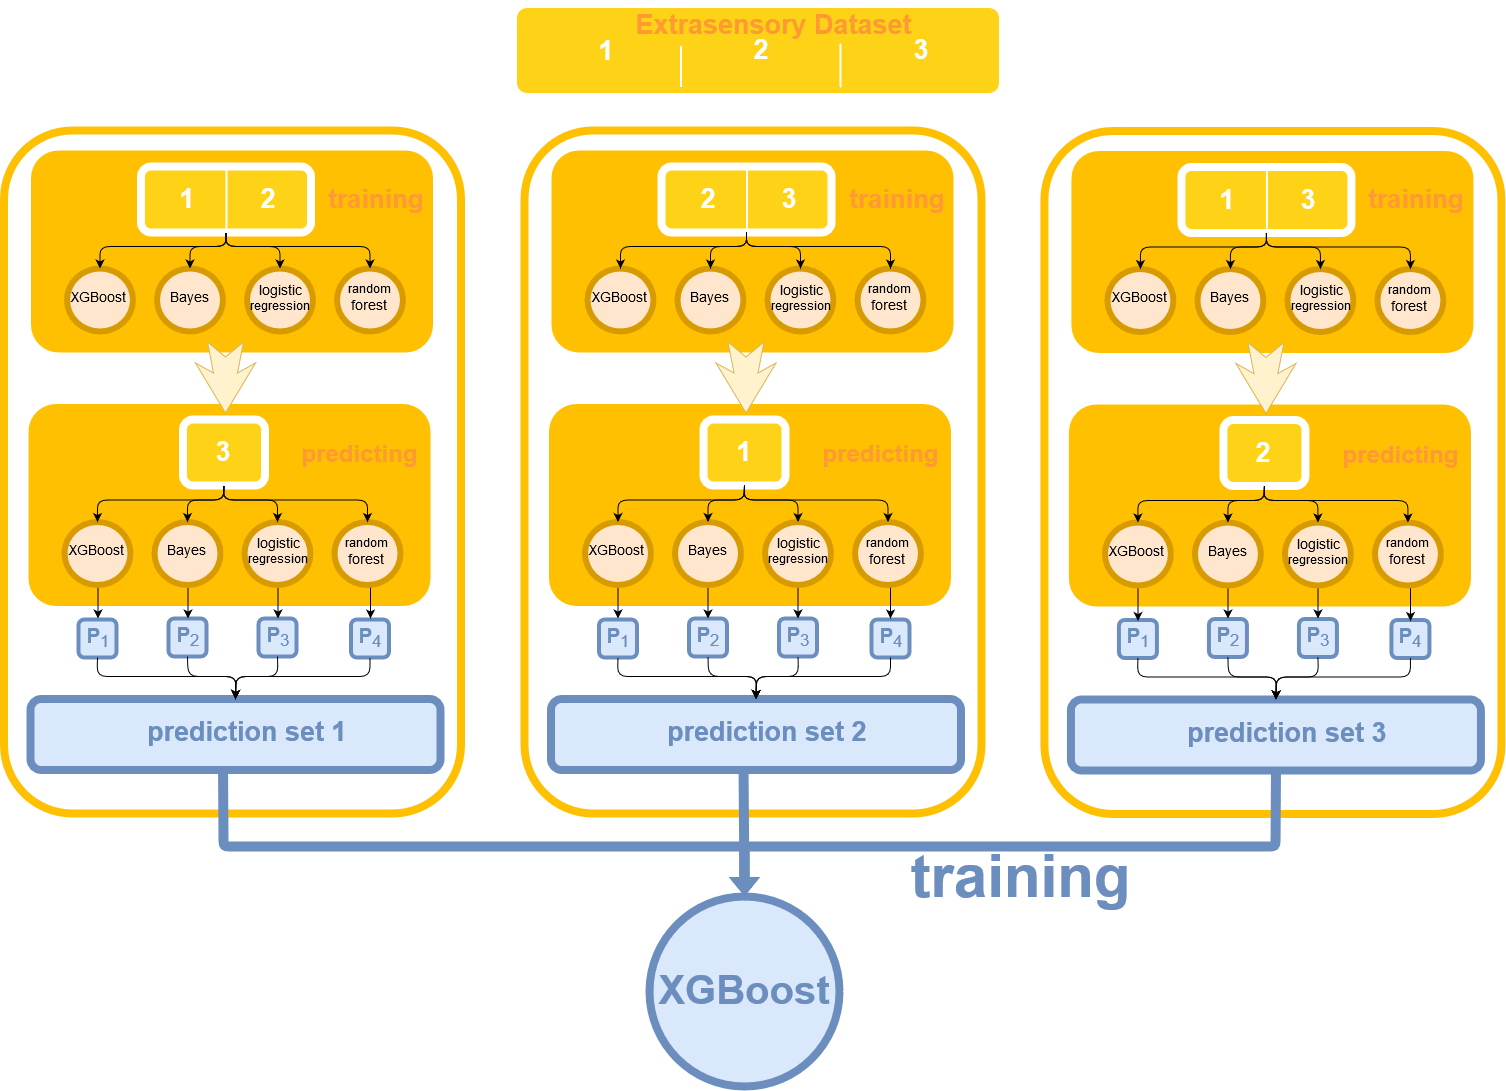
\includegraphics[width=\textwidth]{images/stacking_diagram.png}
		\caption{A Stacking Visualization}
		\label{abb:stacking}
	\end{center}		
\end{figure}	

In our case we used XGBoost, a naive bayes classifier, a random-forest classifier and a linear regression classificator as first-level classifiers and XGBoost as the second-level classificator. As shown in Fig. \ref{abb:stacking}, the first-level classifiers were trained with the principle of Cross Validation, this Stacking technique is also called Cross Validation Stacking, in which the data set was divided by three, resulting in three prediction sets. On these prediction sets, supplemented by the original labels, the training of the second-level classifier took place.

Die Ergänzung des \textcolor{red}{Cross-Validation} Aspekts gegenüber der 